\documentclass{beamer}
\mode<presentation> {
\usepackage{color}
\definecolor{bottomcolour}{rgb}{0.21,0.11,0.21}
\definecolor{middlecolour}{rgb}{0.21,0.11,0.21}
\setbeamercolor{structure}{fg=white}
\setbeamertemplate{frametitle}[default]%[center]
\setbeamercolor{normal text}{bg=black, fg=white}
\setbeamertemplate{background canvas}[vertical shading]
[bottom=bottomcolour, middle=middlecolour, top=black]
\setbeamertemplate{items}[circle]
\setbeamertemplate{navigation symbols}{} %no nav symbols
\setbeamercolor{block title}{use=structure,fg=white,bg=structure.fg!50!red!50!blue!100!green}
\setbeamercolor{block body}{parent=normal text,use=block title,bg=block title.bg!5!white!10!bg,fg=white}
\setbeamertemplate{navigation symbols}{}
}

\usepackage{graphicx} 
\usepackage{booktabs} 
\usepackage[utf8]{inputenc}  
\usepackage[T1]{fontenc}  
\usepackage{geometry}     
\usepackage[francais]{babel} 
\usepackage{eurosym}
\usepackage{verbatim}
\usepackage{ragged2e}
\justifying

%%%%%%%%%%%%%%%%%%%%%%%%%%%%%%%%%%%%%%%%%%%%%%%%%%%%%%%%%%%%%%%%
%% ccBeamer 0.1, 2007-07-02                                   %%
%% Written by Sebastian Pipping <webmaster@hartwork.org>      %%
%% ---------------------------------------------------------- %%
%% Licensed under Creative Commons Attribution-ShareAlike 3.0 %%
%% http://creativecommons.org/licenses/by-sa/3.0/             %%
%%%%%%%%%%%%%%%%%%%%%%%%%%%%%%%%%%%%%%%%%%%%%%%%%%%%%%%%%%%%%%%%


%% Images
\newcommand{\CcImageBy}[1]{%
	
\includegraphics[scale=#1]{creative_commons/cc_by_30.pdf}%
}
\newcommand{\CcImageCc}[1]{%
	
\includegraphics[scale=#1]{creative_commons/cc_cc_30.pdf}%
}
\newcommand{\CcImageDevNations}[1]{%
	
\includegraphics[scale=#1]{creative_commons/cc_dev_nations_30.pdf}%
}
\newcommand{\CcImageNc}[1]{%
	
\includegraphics[scale=#1]{creative_commons/cc_nc_30.pdf}%
}
\newcommand{\CcImageNd}[1]{%
	
\includegraphics[scale=#1]{creative_commons/cc_nd_30.pdf}%
}
\newcommand{\CcImagePd}[1]{%
	
\includegraphics[scale=#1]{creative_commons/cc_pd_30.pdf}%
}
\newcommand{\CcImageSa}[1]{%
	
\includegraphics[scale=#1]{creative_commons/cc_sa_30.pdf}%
}
\newcommand{\CcImageSampling}[1]{%
	
\includegraphics[scale=#1]{creative_commons/cc_sampling_30.pdf}%
}
\newcommand{\CcImageSamplingPlus}[1]{%
	
\includegraphics[scale=#1]{creative_commons/cc_sampling_plus_30.pdf}%
}


%% Groups
\newcommand{\CcGroupBy}[1]{% zoom
	\CcImageBy{#1}%
}
\newcommand{\CcGroupByNc}[2]{% zoom, gap
	\CcImageBy{#1}\hspace*{#2}\CcImageNc{#1}%
}
\newcommand{\CcGroupByNcNd}[2]{% zoom, gap
	\CcImageBy{#1}\hspace*{#2}\CcImageNc{#1}\hspace*{#2}\CcImageNd{#1}%
}
\newcommand{\CcGroupByNcSa}[2]{% zoom, gap
	\CcImageBy{#1}\hspace*{#2}\CcImageNc{#1}\hspace*{#2}\CcImageSa{#1}%
}
\newcommand{\CcGroupByNd}[2]{% zoom, gap
	\CcImageBy{#1}\hspace*{#2}\CcImageNd{#1}%
}
\newcommand{\CcGroupBySa}[2]{% zoom, gap
	\CcImageBy{#1}\hspace*{#2}\CcImageSa{#1}%
}
\newcommand{\CcGroupDevNations}[1]{% zoom
	\CcImageDevNations{#1}%
}
\newcommand{\CcGroupNcSampling}[2]{% zoom, gap
	\CcImageNc{#1}\hspace*{#2}\CcImageSampling{#1}%
}
\newcommand{\CcGroupPd}[1]{% zoom
	\CcImagePd{#1}%
}
\newcommand{\CcGroupSampling}[1]{% zoom
	\CcImageSampling{#1}%
}
\newcommand{\CcGroupSamplingPlus}[1]{% zoom
	\CcImageSamplingPlus{#1}%
}


%% Text
\newcommand{\CcLongnameBy}{Attribution}
\newcommand{\CcLongnameByNc}{Attribution-NonCommercial}
\newcommand{\CcLongnameByNcNd}{Attribution-NoDerivs}
\newcommand{\CcLongnameByNcSa}{Attribution-NonCommercial-ShareAlike}
\newcommand{\CcLongnameByNd}{Attribution-NoDerivs}
\newcommand{\CcLongnameBySa}{Attribution-ShareAlike}

\newcommand{\CcNote}[1]{% longname
	This work is licensed under the \textit{Creative Commons #1 3.0 License}.%
}


\title[Cryptocat]{Cryptocat} 
\author{Genma}

\begin{document}

%% Titlepage
\begin{frame}
	\titlepage
	\vfill
	\begin{center}
		\CcGroupByNcSa{0.83}{0.95ex}\\[2.5ex]
		{\tiny\CcNote{\CcLongnameByNcSa}}
		\vspace*{-2.5ex}
	\end{center}
\end{frame}

%----------------------------------------------------------------------------------------
%	PRESENTATION SLIDES
%----------------------------------------------------------------------------------------
\begin{frame}
\frametitle{
\includegraphics[scale=0.4]{./images/Genma.jpg} \ \ \  A propos de moi  }
\begin{columns}[c] 

\column{.55\textwidth} 
\textbf{Où me trouver sur Internet?}
\begin{itemize}
\item Le Blog de Genma : http://genma.free.fr
\item Twitter : http://twitter.com/genma
\end{itemize}

\textbf{Mes centres d'intérêts?}
\\ Plein de choses dont:
\begin{itemize}
\item La veille technologique
\item Le chiffrement
\end{itemize}
\column{.5\textwidth} 
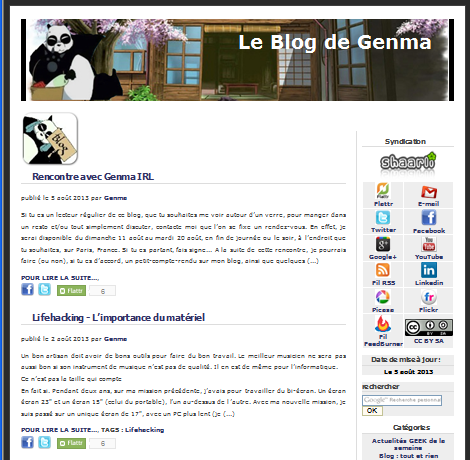
\includegraphics[width=5cm,height=5cm]{./images/blog.png} 
\end{columns}
\end{frame}

%----------------------------------------------------------------------------------------
\begin{frame}
\frametitle{Qu'est ce que Cryptocat}
\begin{itemize}
\justifying{
\item Cryptocat est une application web open source destinée à permettre des communications sûres et chiffrées. 
\item Cryptocat chiffre les chat côté client ; la confiance au serveur se limite à des données déjà chiffrées. 
\item Cryptocat est une extension pour Mozilla Firefox, Google Chrome et Safari, ainsi qu'une application Mac OSX native.  
}
\end{itemize}	
\end{frame}

%------------------------------------------------
\begin{frame}
\frametitle{}
\begin{center}
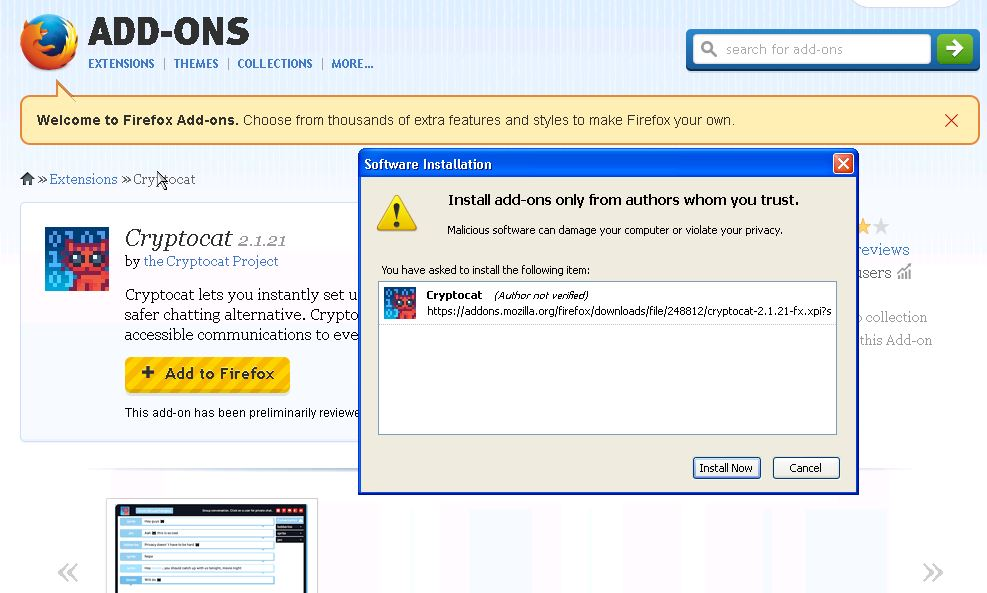
\includegraphics[scale=0.5] {./images/Cryptocat01.jpg} 
\end{center}
\end{frame}

%----------------------------------------------------------------------------------------
\begin{frame}
\frametitle{Cryptocat en extension Firefox}
\begin{itemize}
\justifying{
\item Cryptocat s'installe donc comme une extension Firefox et au premier lancement, il est indiqué que l'on aura un icone dans la barre de menu.
}
\end{itemize}	
\end{frame}

%------------------------------------------------
\begin{frame}
\frametitle{}
\begin{center}
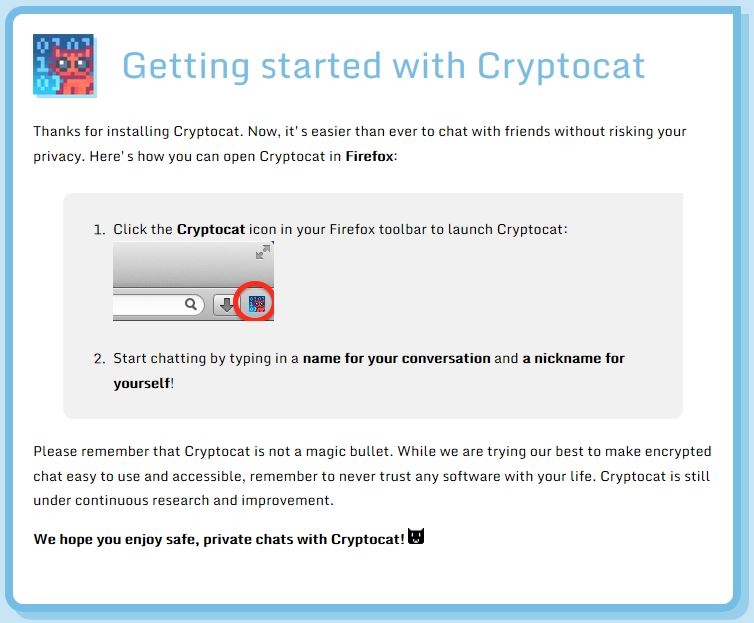
\includegraphics[scale=0.5] {./images/Cryptocat02.jpg} 
\end{center}
\end{frame}

%----------------------------------------------------------------------------------------
\begin{frame}
\frametitle{Cryptocat - lancement d'une conversation}

\justifying{Une fois que l'on clique sur l'icone de Cryptocat, on a la fenêtre suivante :}
\begin{itemize}
\justifying{
\item On saisit le nom d'une conversation (que l'on veut créer ou rejoindre).
\item On saisit un pseudonyme.
\item On clique sur connexion.
}
\end{itemize}	
\end{frame}

%------------------------------------------------
\begin{frame}
\frametitle{}
\begin{center}
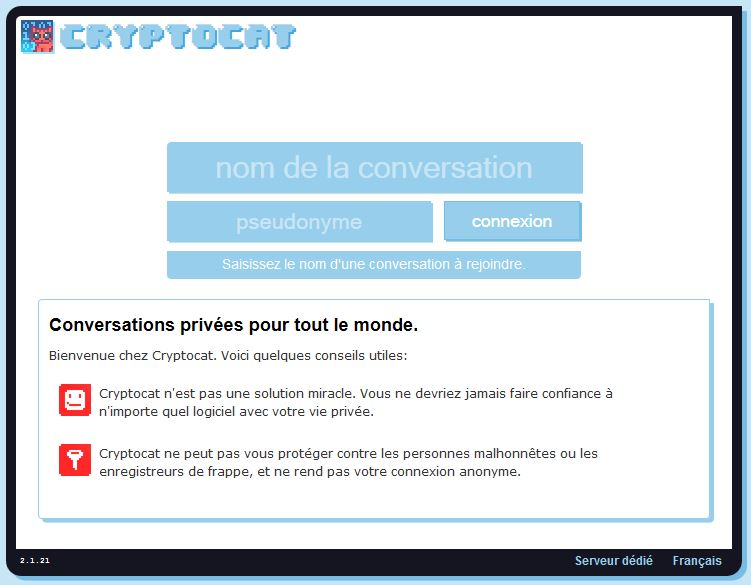
\includegraphics[scale=0.5] {./images/Cryptocat03.jpg} 
\end{center}
\end{frame}

%------------------------------------------------
\begin{frame}
\frametitle{}
\begin{center}
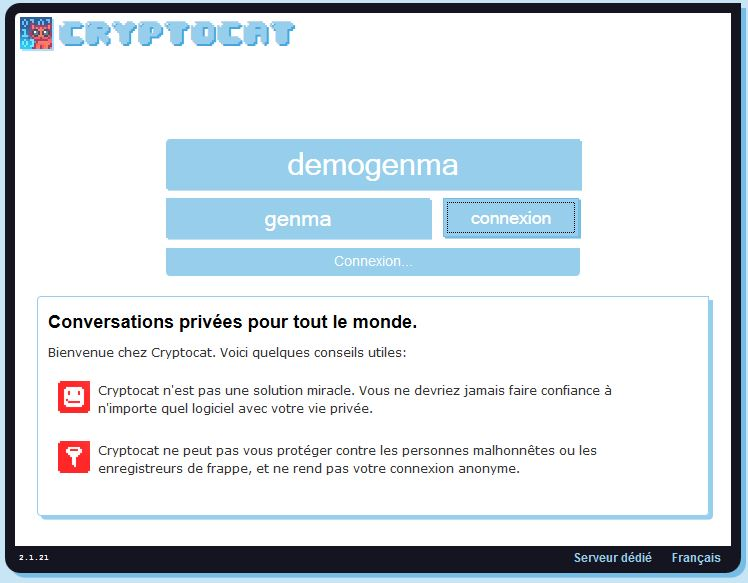
\includegraphics[scale=0.5] {./images/Cryptocat04.jpg} 
\end{center}
\end{frame}

%------------------------------------------------
\begin{frame}
\frametitle{}
\begin{center}
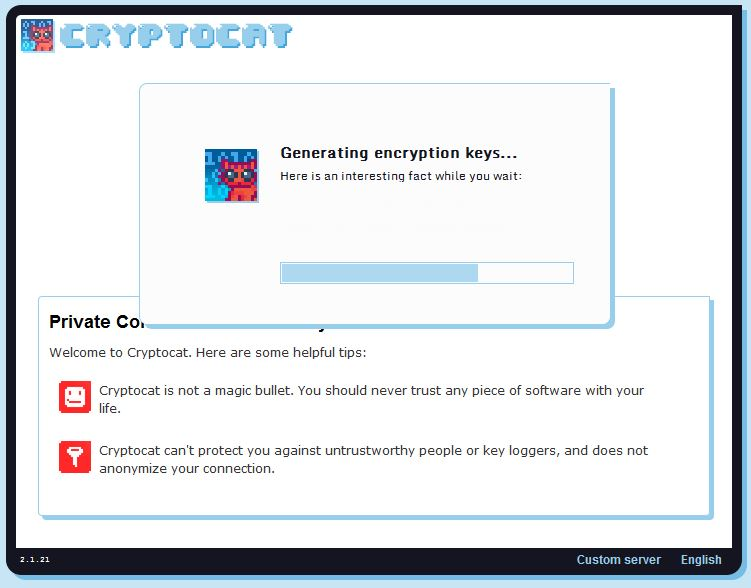
\includegraphics[scale=0.5] {./images/Cryptocat05.jpg} 
\end{center}
\end{frame}

%----------------------------------------------------------------------------------------
\begin{frame}
\frametitle{Cryptocat - début d'une conversation}

\justifying{}
\begin{itemize}
\justifying{
\item La communication est alors établie de façon chiffrée.
\item Dans l'exemple, Genma voit que Ryoga est connecté.
\item Ryoga lui a envoyé un message, auquel Genma réponds.
}
\end{itemize}	
\end{frame}


%------------------------------------------------
\begin{frame}
\frametitle{}
\begin{center}
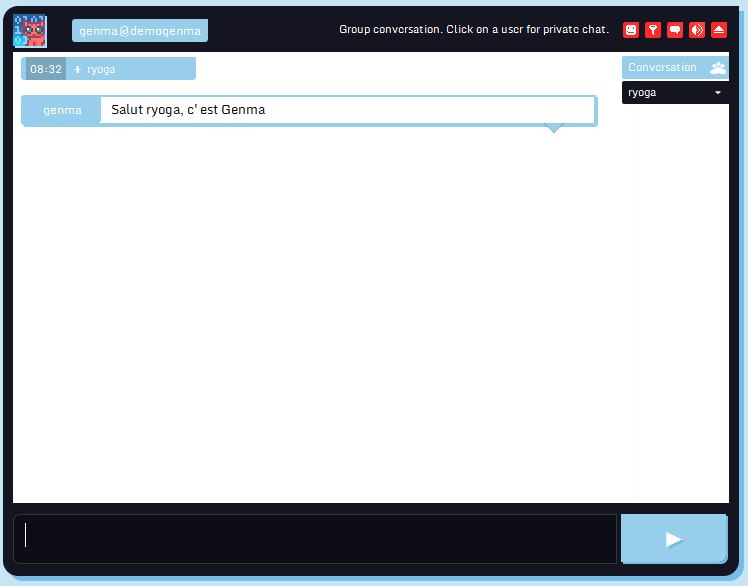
\includegraphics[scale=0.5] {./images/Cryptocat06.jpg} 
\end{center}
\end{frame}

%------------------------------------------------
\begin{frame}
\frametitle{}
\begin{center}
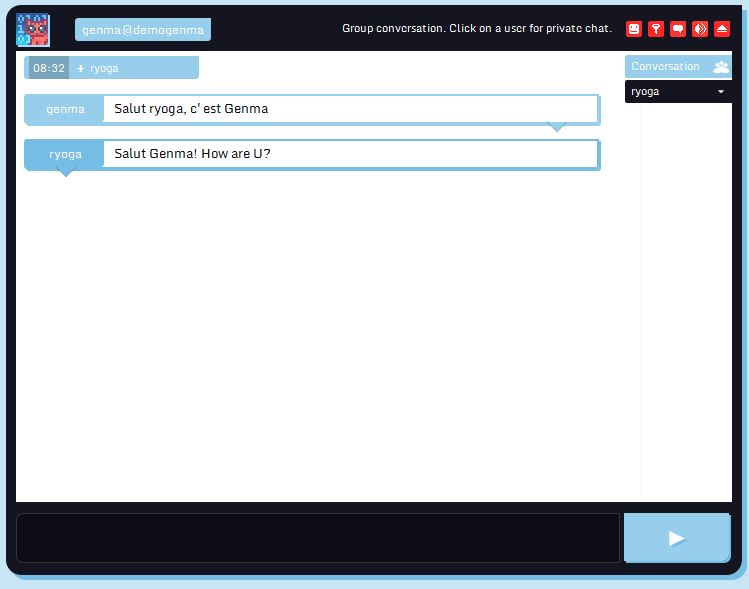
\includegraphics[scale=0.5] {./images/Cryptocat07.jpg} 
\end{center}
\end{frame}

%----------------------------------------------------------------------------------------
\begin{frame}
\frametitle{Cryptocat - conversation en cours}

\justifying{}
\begin{itemize}
\justifying{
\item Quand un participant est en train de rédiger un texte, un icone l'indique sur l'écran des autres participants. 
}
\end{itemize}	
\end{frame}

%------------------------------------------------
\begin{frame}
\frametitle{}
\begin{center}
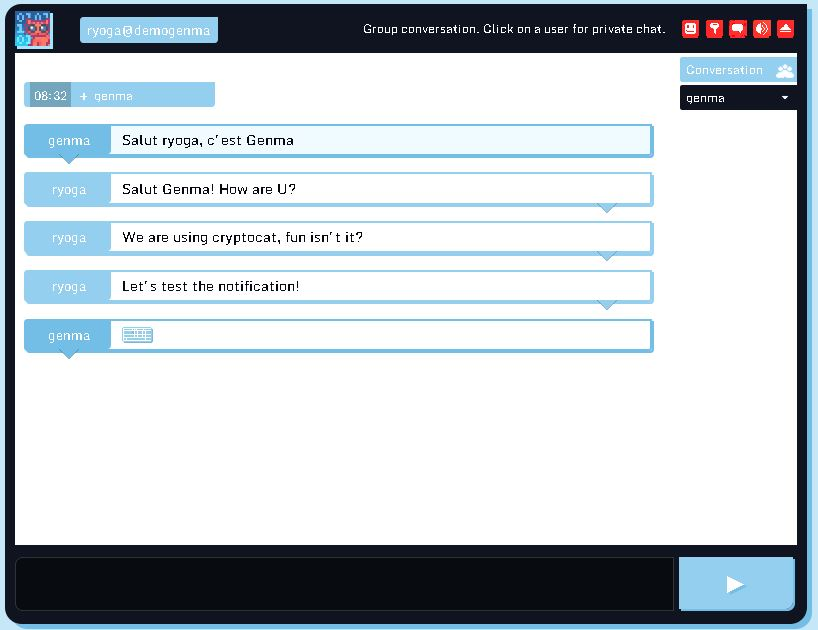
\includegraphics[scale=0.5] {./images/Cryptocat08.jpg} 
\end{center}
\end{frame}

%----------------------------------------------------------------------------------------
\begin{frame}
\frametitle{Cryptocat - validation des participants}

\justifying{Dans la barre de menu}
\begin{itemize}
\justifying{
\item Quand on clique sur l'icône myInfo, on a différentes informations.
\item En particulier le "group conversation fingerprints".
\item Et le OTR fingerprint.
}
\end{itemize}	
\end{frame}

%------------------------------------------------
\begin{frame}
\frametitle{}
\begin{center}
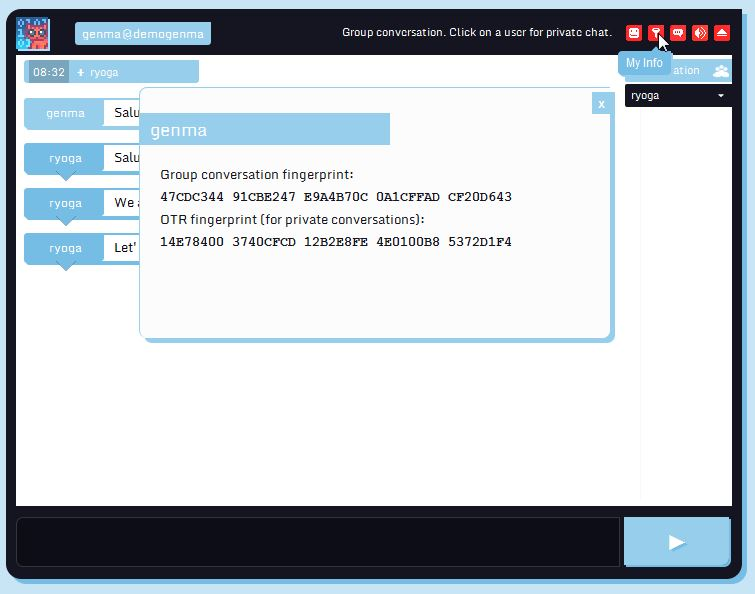
\includegraphics[scale=0.5] {./images/Cryptocat09.jpg} 
\end{center}
\end{frame}

%----------------------------------------------------------------------------------------
\begin{frame}
\frametitle{Cryptocat - validation des participants}

\justifying{Quand on clique sur le nom d'un participant}
\begin{itemize}
\justifying{
\item On retrouve les mêmes informations.
\item Il est possible de saisir une question secrète
\item Et la réponse à cette question.
}
\end{itemize}	
\justifying{On transemttra la réponse au participant via un autre canal de communication.}
\end{frame}

%------------------------------------------------
\begin{frame}
\frametitle{}
\begin{center}
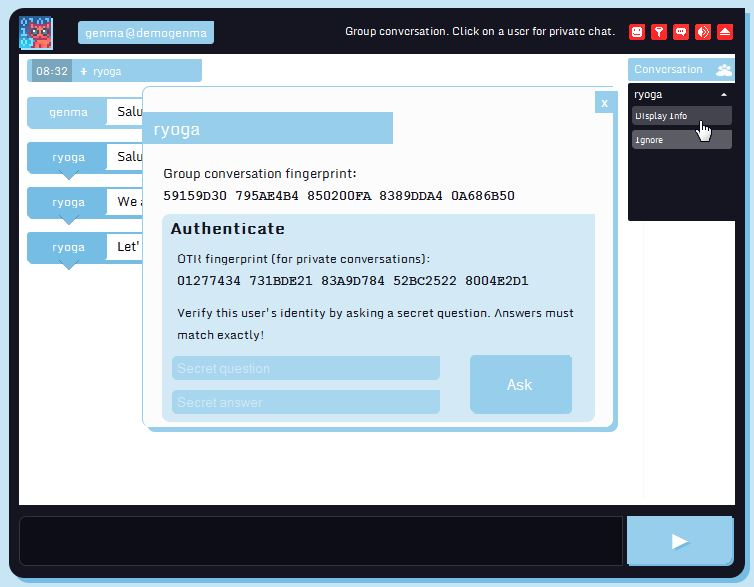
\includegraphics[scale=0.5] {./images/Cryptocat10.jpg} 
\end{center}
\end{frame}

%----------------------------------------------------------------------------------------
\begin{frame}
\frametitle{Cryptocat - validation des participants}

\justifying{Sur l'écran de l'autre participant (Ryoga)}
\begin{itemize}
\justifying{
\item Celui-ci se voit demander la réponse à la question secrète.
\item Il saisit la réponse qu'il connait.
}
\end{itemize}	
\end{frame}

%------------------------------------------------
\begin{frame}
\frametitle{}
\begin{center}
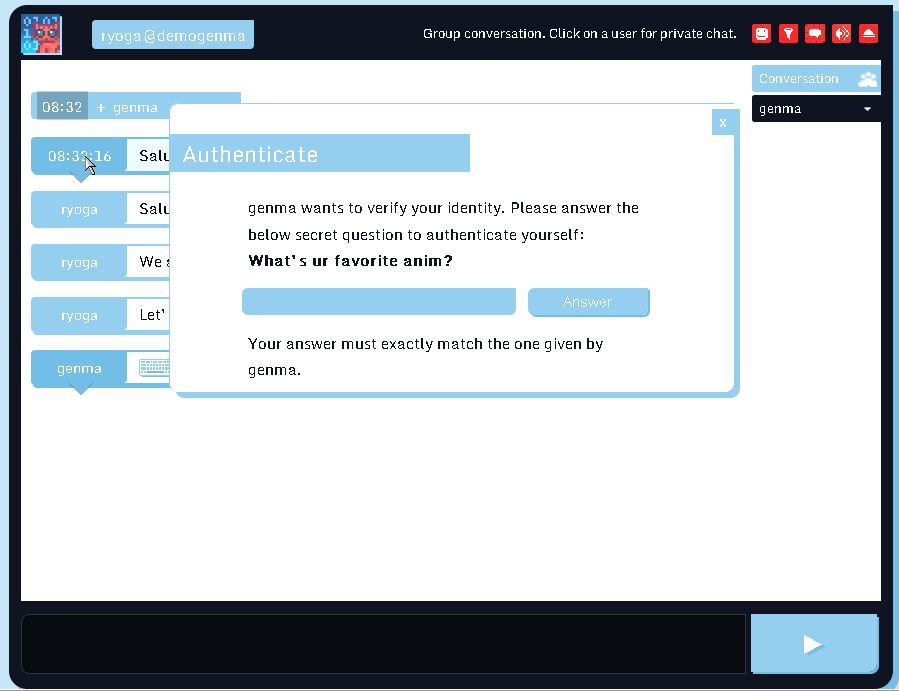
\includegraphics[scale=0.5] {./images/Cryptocat11.jpg} 
\end{center}
\end{frame}

%----------------------------------------------------------------------------------------
\begin{frame}
\frametitle{Cryptocat - validation des participants}

\justifying{Sur l'écran de Genma}
\begin{itemize}
\justifying{
\item Il y a un message qui indique Ryoga a bien saisit la bonne réponse.
\item On a une validation que la personne qui utilise le pseudonyme de Ryoga est bien celle qu'elle prétend être.
}
\end{itemize}	
\end{frame}

%------------------------------------------------
\begin{frame}
\frametitle{}
\begin{center}
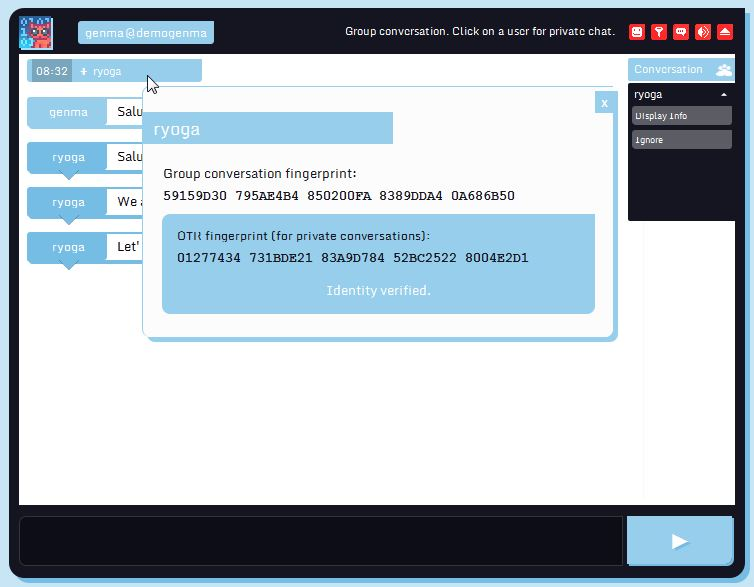
\includegraphics[scale=0.5] {./images/Cryptocat12.jpg} 
\end{center}
\end{frame}

%----------------------------------------------------------------------------------------
\begin{frame}
\frametitle{Cryptocat - validation des participants}

\justifying{}
\begin{itemize}
\justifying{
\item Ryoga posera à son  tour une question secrète si besoin, pour valider l'identité de Genma.
}
\end{itemize}	
\end{frame}

\end{document}